\documentclass[11pt, a4paper]{article}

\usepackage{amsmath}
\usepackage{pgf}
\usepackage{tikz}
\usepackage{kbordermatrix}
\usetikzlibrary{arrows,automata, shapes, petri}
\usepackage{placeins}
\usepackage{multirow}
\usepackage{booktabs}

\begin{document}

\title{HIDDEN MARKOV MODELS}
\date{}
\maketitle

Hidden Markov Models(HMMs) are statistical tools to model sequential observations with the assumption that states of the system generating them follow a Markov process but these states are unobservable/hidden. However, an observation at any point is related to the underlying hidden state the system is in at that point.

\section{Example}

\begin{center}
	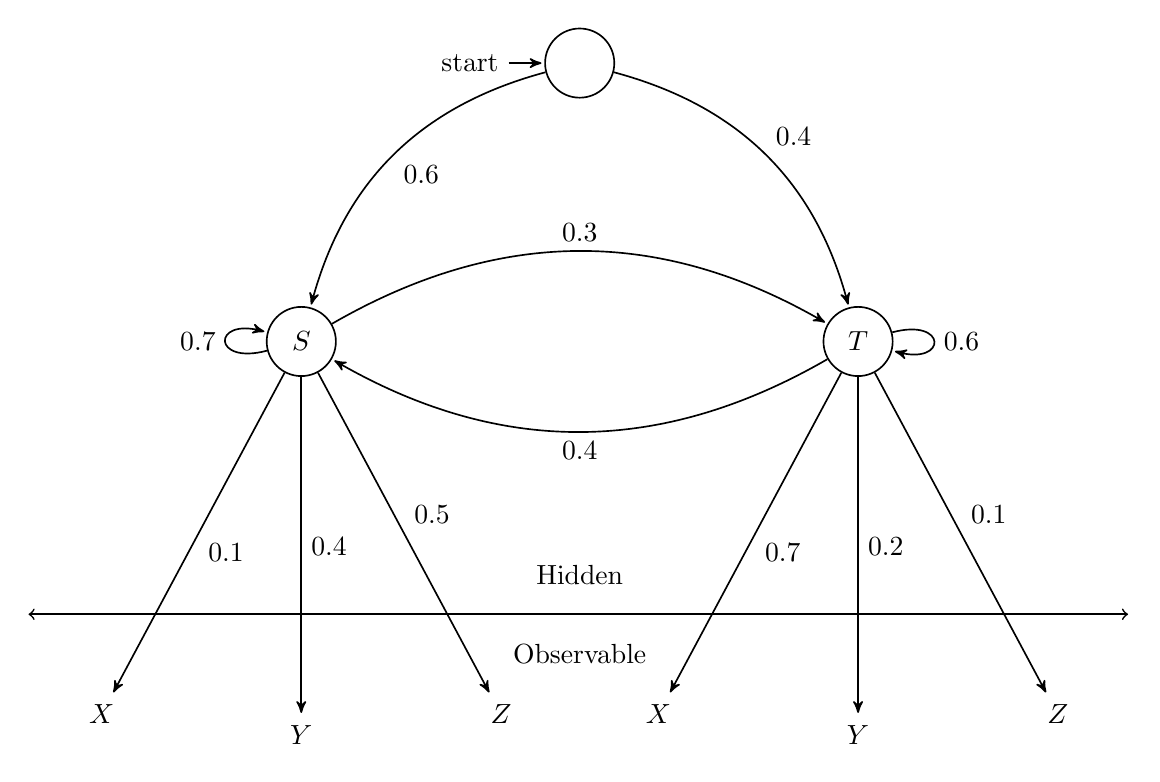
\begin{tikzpicture}[->,>=stealth',shorten >=1pt,auto,node distance=5cm,
		semithick]
		
		\node[initial,state] (I)                    {$$};
		\node[state]         (S) [below left of=I] {$S$};
		\node[state]         (T) [below right of=I] {$T$};
		\node[rectangle]         (SX) [below left of=S,yshift=-1.2cm,xshift=1cm]     {$X$};
		\node[rectangle]         (SY) [below of=S]     {$Y$};  
		\node[rectangle]         (SZ) [below right of=S,yshift=-1.2cm,xshift=-1cm]     {$Z$};
		\node[rectangle]         (TX) [below left of=T,yshift=-1.2cm,xshift=1cm]     {$X$};
		\node[rectangle]         (TY) [below of=T]     {$Y$};  
		\node[rectangle]         (TZ) [below right of=T,yshift=-1.2cm,xshift=-1cm]     {$Z$};  
		
		\path (I) edge [bend right]    node {0.6} (S)
		edge [bend left]     node {0.4} (T)
		(S) edge [loop left]    node {0.7} (S)
		edge [bend left]    node {0.3} (T)
		edge                node {0.1} (SX)
		edge                node {0.4} (SY)
		edge                node {0.5} (SZ)
		(T) edge [loop right]   node {0.6} (T)
		edge [bend left]    node {0.4} (S)
		edge                node {0.7} (TX)
		edge                node {0.2} (TY)
		edge                node {0.1} (TZ);   
		\draw [to-to] (-7,-7) -- (7,-7); 
		\node at (0, -6.5) {Hidden};
		\node at (0, -7.5) {Observable};                   
	\end{tikzpicture}
\end{center}

In this diagram, nodes $\{S, T\}$ represent the hidden states and $\{X, Y, Z\}$ represent observable states. The unlabelled node is the start node. These states together with the associated probabilities fully characterize the HMM. The state transition probabilites denoted by A can be represented as,

\[
	A = \kbordermatrix{
		& S & T \\
		S & 0.7 & 0.3 \\
		T & 0.6 & 0.4 \\
	}
\]

The emmission probabilities are denoted by B.

\[
	B = \kbordermatrix{
		& X & Y & Z \\
		S & 0.1 & 0.4 & 0.5 \\
		T & 0.7 & 0.2 & 0.1 \\
	}
\]

Lastly, initial state distribution is denoted by $\pi$.

\[
	\pi = \kbordermatrix{
		& S & T \\
		& 0.6 & 0.4  
	}
\]

\section{The three problems of HMM}

\subsection{The Evaluation Problem}

Given a HMM, $\lambda=(A, B, \pi)$ and a set of observations $O$, find $P(O|\lambda)$ (probability that the observations were generated by the model).

Consider the HMM in the example above and let $O = (ZXY)$.

\begin{align*}
	P(ZXY|\lambda) & = P(SSS, ZXY|\lambda)  \\
	               & +\ P(SST, ZXY|\lambda) \\
	               & +\ P(STS, ZXY|\lambda) \\
	               & +\ P(STT, ZXY|\lambda) \\
	               & +\ P(TSS, ZXY|\lambda) \\
	               & +\ P(TST, ZXY|\lambda) \\
	               & +\ P(TTS, ZXY|\lambda) \\
	               & +\ P(TTT, ZXY|\lambda) \\  
\end{align*}

Each of the terms on R.H.S. can be calculated using the following law of probability.

\begin{align*}
	P(a, b|c) & = \frac{P(a, b, c) }{P(c)}                            \\ 
	          & = \frac{P(a, c) }{P(c)} * \frac{P(a, b, c) }{P(a, c)} \\
	          & = P(a|c) * P(b|a,c)                                   
\end{align*} 

\begin{table}[h!]
	\centering
	\caption{$P(ZXY|\lambda)$ calculation}
	\label{tab:table1}
	\begin{tabular}{cccc|c}
		\toprule
		HS  & OS  & $P(HS|\lambda)$   & $P(OS|HS, \lambda)$ & $P(HS, OS|\lambda)$ \\
		\midrule
		SSS & ZXY & 0.6*0.7*0.7=0.294 & 0.5*0.1*0.4=0.020   & 0.005880            \\
		SST & ZXY & 0.6*0.7*0.3=0.126 & 0.5*0.1*0.2=0.010   & 0.001260            \\
		STS & ZXY & 0.6*0.3*0.4=0.072 & 0.5*0.7*0.4=0.140   & 0.010080            \\
		STT & ZXY & 0.6*0.3*0.6=0.108 & 0.5*0.7*0.2=0.070   & 0.007560            \\
		TSS & ZXY & 0.4*0.4*0.7=0.112 & 0.1*0.1*0.4=0.004   & 0.000448            \\
		TST & ZXY & 0.4*0.4*0.3=0.048 & 0.1*0.1*0.2=0.002   & 0.000096            \\
		TTS & ZXY & 0.4*0.6*0.4=0.096 & 0.1*0.7*0.4=0.028   & 0.002688            \\
		TTT & ZXY & 0.4*0.6*0.6=0.144 & 0.1*0.7*0.2=0.014   & 0.002016            \\
		\midrule
		    &     &                   & $P(ZXY|\lambda)$    & 0.030028            \\
		\bottomrule
	\end{tabular}
\end{table}

Calculation in this manner is expensive because probabilities corresponding to all permutations of hidden states of the same length as the length of observed sequence have to be calculated. 

\subsection{The Decoding Problem}

\subsection{The Learning Problem}


\end{document}